% Copyright 2004 by Till Tantau <tantau@users.sourceforge.net>.
%
% In principle, this file can be redistributed and/or modified under
% the terms of the GNU Public License, version 2.
%
% However, this file is supposed to be a template to be modified
% for your own needs. For this reason, if you use this file as a
% template and not specifically distribute it as part of a another
% package/program, I grant the extra permission to freely copy and
% modify this file as you see fit and even to delete this copyright
% notice. 
\def\ACCOMPLETE{}
\documentclass{beamer}
\usepackage{color}
\usepackage{graphicx}
\usepackage{marvosym}
\usepackage{tikz}
\usepackage{multirow}
\setbeamertemplate{items}[circle]
\setbeamercovered{transparent}

\usetheme{Madrid}
\newcommand{\mc}{\mathcal}
\newcommand{\mb}{\mathbf}
\newcommand{\tr}{\text{Tr}}
\newcommand\numberthis{\addtocounter{equation}{1}\tag{\theequation}}
\let\oldnl\nl
\newcommand{\nonl}{\renewcommand{\nl}{\let\nl\oldnl}}

\DeclareMathOperator*{\argmin}{arg\,min}
\DeclareMathOperator*{\vcdim}{VC-Dim}

\newcommand\mynum[1]{%
  \usebeamercolor{enumerate item}%
  \tikzset{beameritem/.style={circle,inner sep=0,minimum size=2ex,text=enumerate item.bg,fill=enumerate item.fg,font=\footnotesize}}%
  \tikz[baseline=(n.base)]\node(n)[beameritem]{#1};%
}

\def\checkmark{\tikz\fill[scale=0.4](0,.35) -- (.25,0) -- (1,.7) -- (.25,.15) -- cycle;} 


\title[Efficient Clustering]{Theoretical foundations for efficient clustering}

\author[S. Kushagra]{
Shrinu Kushagra\\
\vspace{30pt}Ph.D Thesis Presentation\\
University of Waterloo
}
\date{\today}

\AtBeginSubsection[]
{
  \begin{frame}<beamer>
  \frametitle{Outline}
    \tableofcontents[currentsection]
  \end{frame}
}

% Let's get started
\begin{document}

\begin{frame}
  \titlepage
\end{frame}

\begin{frame}{What is clustering?}
	Given: $(X, d)$\\
	\vspace{10pt}Partition it into $k$ subsets .$$C = \{C_1, \ldots, C_k\}$$
	\begin{itemize}
		\item Similar points share a cluster.
		\item Dis-similar points are separated.
	\end{itemize}
\end{frame}

\begin{frame}<1-2>[label=clusteringChallenges]{Challenges in clustering}
	\begin{enumerate}
		\onslide<1> \item Computational complexity
			\begin{itemize}
				\vspace{10pt}\item Optimization problem 
				\vspace{10pt}\item \hyperlink{notesIntroduction}{NP-Hard for common functions like $k$-means, $k$-median.}
			\end{itemize}
		\onslide<2> \vspace{20pt}\item  Under-specificity
		\onslide<3>\vspace{20pt}\item Noise robustness
	\end{enumerate}

\end{frame}


\begin{frame}{Under-specificity in clustering}
	
	Requirements from clustering algorithms\\
	\vspace{10pt}
	\begin{block}{}
		\begin{itemize}
			\item Similar points together
			\item Dis-similar points separated
		\end{itemize}
	\end{block}
	
	\vspace{10pt}\alert{Conflicting}
	\begin{center}
	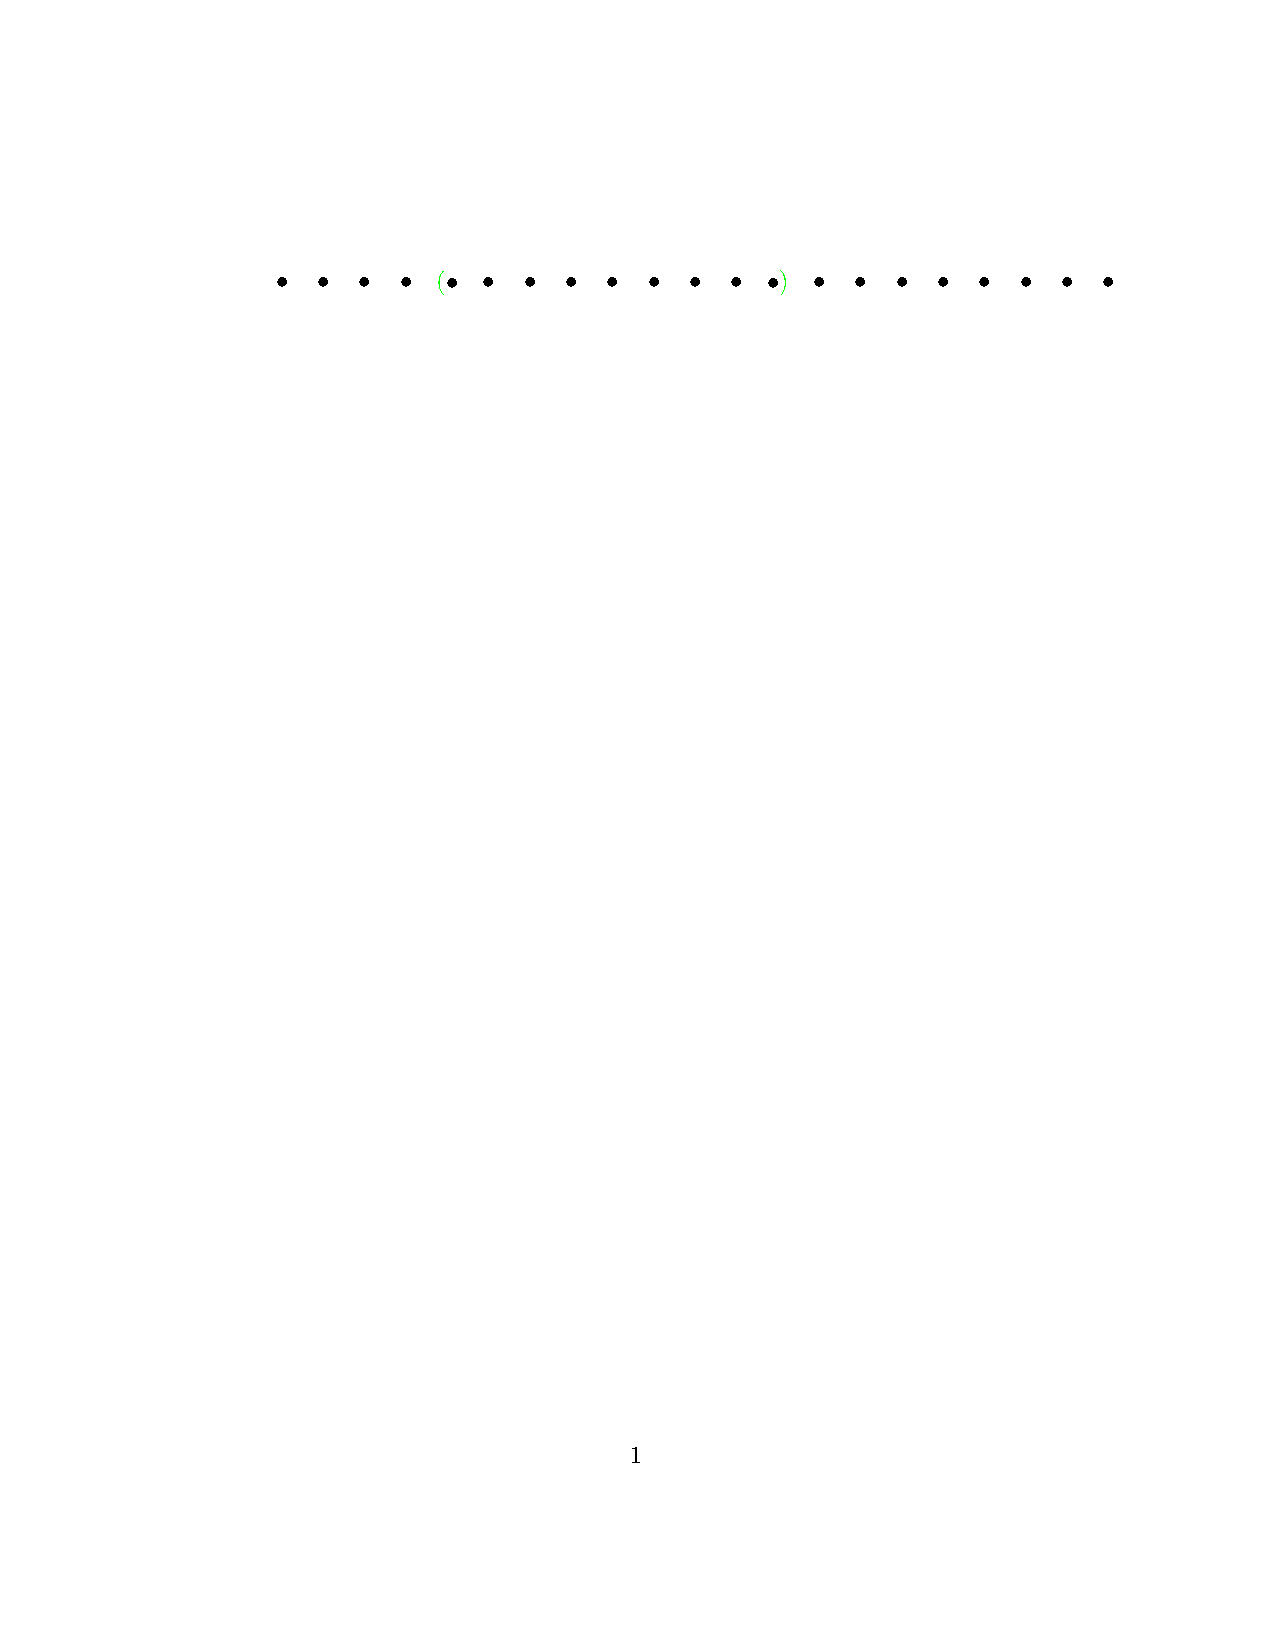
\includegraphics[trim={100 650 30 120},clip,width=0.8\textwidth]{figures/conflictingReq.pdf}
	\end{center}
\end{frame}

\begin{frame}{Different algorithms, different considerations}
	Given $X \in \mb R^2$ and $k = 2$
	\begin{center}
	\begin{figure}
	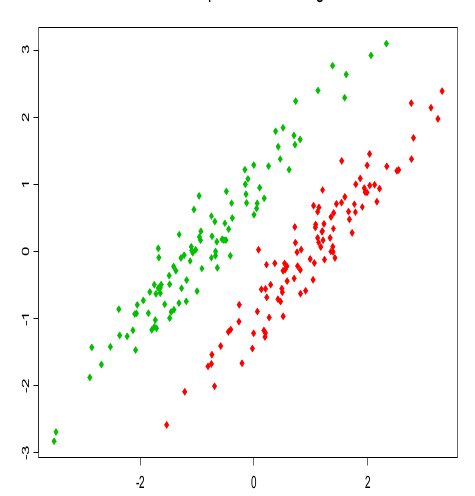
\includegraphics[trim={0 0 0 20},clip,width=0.4\textwidth]{figures/slX.png}
	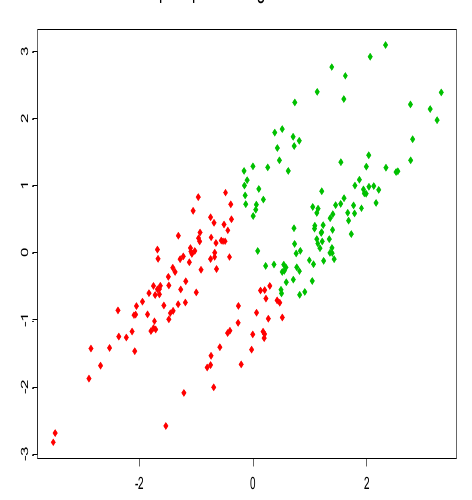
\includegraphics[trim={0 0 0 20},clip,width=0.4\textwidth]{figures/kmeansX.png}
	\caption{Single-linkage on our example dataset (Left). $k$-means on our example dataset (Right)}
	\end{figure}
	\end{center}
\end{frame}

\begin{frame}{Model selection problem}
	
	 Under-specificity\\
	\begin{itemize}
		\vspace{10pt}\item Basic definition \alert{can't} resolve this conflict.
		\vspace{10pt}\item Other requirements: Balance amongst cluster sizes etc. 
	\end{itemize}
	
	\vspace{20pt}\textcolor{blue}{How to prefer one choice over the other}?
\end{frame}

\againframe<3>{clusteringChallenges}

\begin{frame}{Noise-robustness}
	Real world data
	\begin{itemize}
		\vspace{10pt}\item Well-clustered subset
		\vspace{5pt}\item Unstructured part
	\end{itemize}
	
	\vspace{25pt}Can we develop \alert{efficient algorithms to detect the structure in the presence of noise}?
\end{frame}

\begin{frame}<1>{Outline}
	First part
	\vspace{10pt}\begin{block}{}
	\mynum{2} Under-specificity \alert{and} \\\vspace{10pt}\mynum{1} Computational complexity
	\end{block}
		
	\onslide<2>\vspace{35pt}Second part
	\vspace{10pt}\begin{block}{}
	\mynum{3} Noise-robustness \alert{and} \\\vspace{10pt}\mynum{1} Computational complexity
	\end{block}		
\end{frame}

\begin{frame}[label=underspecificityRelated]{Dealing with under-specificity}

	\hyperlink{notesUnderspecificityRelated}{Incorporating domain knowledge into the clustering problem}\\	
	\begin{itemize}
		\vspace{10pt} \item Must/cannot link constraints \alert{[Wagstaff et. al `01]}\\
		\vspace{10pt} \item Demonstration-based clustering \alert{[Ashtiani, Ben-David `15]}\\
		\vspace{10pt} \item Merge/split queries \alert{[Balcan, Blum `08]}
	\end{itemize}
\end{frame}

\begin{frame}{Our approach to tackling under-specificity}
	

    \vspace{20pt}Ask {\color{blue}same-cluster queries} to a $C^*$-oracle\\
    $$C^*(x_1, x_2) = \left\{
	\begin{array}{ll}
		\mbox{true }  & \mbox{if } x_1 \overset{C^*}{\sim} x_2   \\
		\mbox{false } & otherwise 
	\end{array}
\right. $$
\end{frame}

\begin{frame}{Center-based clustering with same-cluster queries}
	\begin{itemize}
		\item Joint work with Hassan Ashtiani and Shai Ben-David
		\vspace{20pt} \item In proceedings of \alert{NeurIPS'16}.
	\end{itemize}
\end{frame}

\begin{frame}{Problem Setting}
	Input: $X \subseteq \mb R^d$, $k$.
	\begin{itemize} 
   		\vspace{10pt}\item Learner can make same-cluster queries to $C^*$-oracle
		\vspace{10pt}\item Oracle's clustering is ``nice"
	\end{itemize}
	\vspace{30pt} {\color{blue}Goal}: Recover the oracle's clustering $C^* = \{C_1^*, \ldots, C_k^*\}$
\end{frame}

\begin{frame}[label=gammaMargin]{$\gamma$-margin niceness}
	\hyperlink{resultsGammaMargin}{Cluster-center is closer to its own points than to points outside}.
	\vspace{1cm}\begin{figure}        
            \centering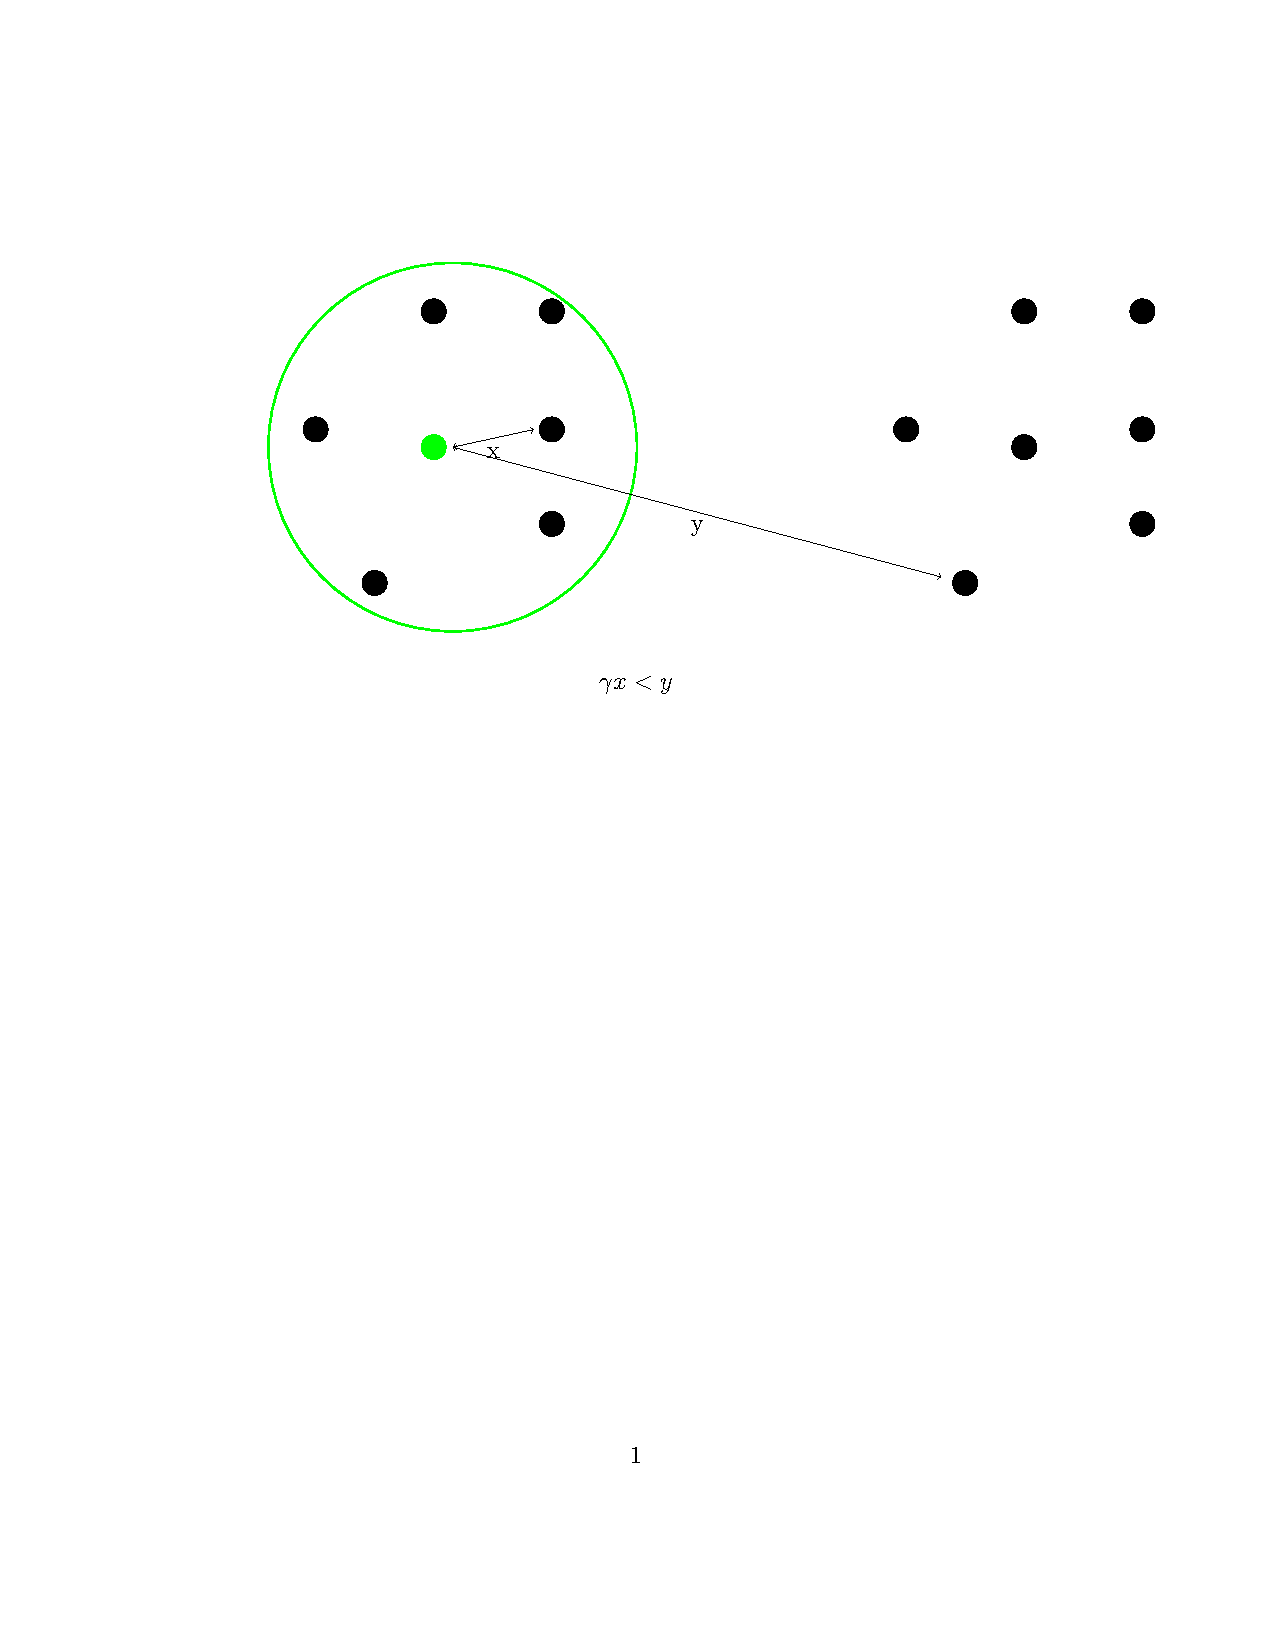
\includegraphics[trim= 400 470 400 150, scale=0.5]{figures/gammaMargin.pdf}
    \end{figure} 
    \begin{block}{}
		For all $i$, for all $x \in C_i$ and for all $y \not\in C_i$
		$$\gamma d(x, \mu_i) < d(y, \mu_i)$$	
	\end{block}  
\end{frame}

\begin{frame}[label=queryPositive]{Results}

	\begin{block}{\hyperlink{resultQueryPositive}{Positive} result with queries}
		\vspace{10pt}For $\gamma > 1$, our algorithm finds $C^*$ (with high probability) and 
		\begin{itemize}
		\vspace{10pt}\item Runs in $O(kn\log n)$ time.
        \vspace{10pt}\item Makes $O(k^2\log k + k\log n)$ same-cluster queries.
		\end{itemize}
	\end{block}
	
	\vspace{20pt}Any target clustering $C^*$ as long the niceness conditions are satisfied. 
\end{frame}

\begin{frame}{$k$-means revisited}
	Input: $X \subseteq \mb R^d$ and $k$.
	\vspace{-10pt}$$C^* = \argmin_{C} \sum_{i=1}^k \sum_{x \in C_i} \|x - \mu_i\|^2$$
	\vspace{10pt}Find $C^*$ given that it satisfies $\gamma$-margin.
	
	\vspace{20pt} {\color{blue}Can efficiently find the optimal using $O(k\log n)$ queries for $\gamma > 1$}
	\begin{center}
		\alert{BUT}
	\end{center}	
	\begin{block}{Theorem}
	Euclidean $k$-means is NP-hard even when the optimal solution satisfies the $\gamma$-margin property for $\gamma < 1.84$
	\end{block}
	
\end{frame}

\begin{frame}[label=queryNegative]{Hardness result}
	\begin{itemize}
		\item \hyperlink{resultQueryNegative}{Reduction from exact cover by $3$-sets ($X3C$)}
		\item Hard for $k = \Theta(n^\epsilon)$ and $d = 2$.
		\item Similar ideas as in \alert{[Vattani'09]}
	\end{itemize}
	
	\begin{figure}
		\centering
		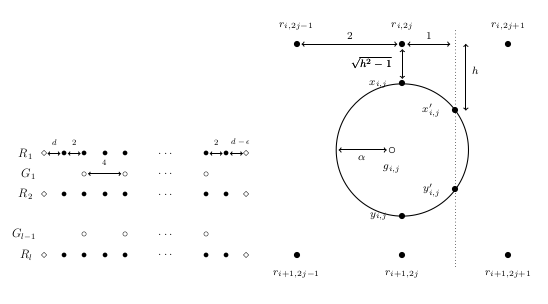
\includegraphics[trim=0 0 0 0,scale=0.5]{figures/hardnessFig.png}
	\end{figure}
\end{frame}

\begin{frame}[label=queryTakeaways]{Key Takeaways}
	
	\begin{itemize}
		\item \hyperlink{notesQueryTakeaways}{Same-cluster queries} tackle under-specificity.
		\vspace{30pt}\item NP-Hard problem becomes {\color{blue}tractable with few queries}. 
	\end{itemize}
\end{frame}


\begin{frame}{Data de-duplication with same-cluster queries}
	\begin{itemize}
		\item Joint work with Shai Ben-David and Ihab Ilyas.
		\vspace{20pt}\item Experiments and hashing based algorithms are joint work with Hemant Saxena.		
		\vspace{20pt} \item In proceedings of \alert{AISTATS'19} and \alert{ICDE'19}.
	\end{itemize}
\end{frame}

\begin{frame}{De-duplication}
	\onslide<1->
    Given a database $X$. \\

    \vspace{10pt}\alert{Detect} records which correspond to the same real-world entity.
    
    \vspace{30pt}Output a clustering of $X$.
\end{frame}

\begin{frame}{Clustering for de-duplication}
	Differences compared to standard formulations\\
    \begin{itemize}
    	\vspace{10pt}\item The number of clusters are given as input. \\
    	For example: $k$-means, $k$-median etc.\\
    	\vspace{10pt}\textcolor{blue}{$k$ is unknown.}
	\end{itemize}    	
\end{frame}

\begin{frame}[label=CC]{Correlation clustering (CC) for de-duplication}
	Input: $X$\\
	Distance   : $d$ over $X^2$\\
	\begin{itemize}
		\item \hyperlink{notesCC}{User designed} (prior knowledge of domain) 
		\item Learned from labelled data.
	\end{itemize}
	 
	\vspace{20pt}Graph $G = (X, E)$. \\
    \vspace{10pt}\hyperlink{notesCCHardness}{Find a clustering which minimizes}
    
    \begin{center}
    \textcolor{blue}{\# zero edges within a cluster + \# one edges\\ across different clusters}
    \end{center}
    
\end{frame}

\begin{frame}[label=CCFramework]{CC framework: Missing pieces}
	\hyperlink{CCThoughts}{Extra information}
    \begin{itemize}
    	\vspace{10pt}\item Easy if $E$ corresponds to a clustering.\\
    	\vspace{10pt}\item What if the optimal solution is `close to' $E$ ? 
	\end{itemize}
	
	\onslide<2->
	\vspace{30pt}Applicability of same-cluster queries.
	
\end{frame}

\begin{frame}{Promise Correlation Clustering (PCC)}
	\begin{block}{Input}
		$G = (X, E)$
	\end{block}
	
	\begin{block}{Find}
	\vspace{-15pt}\begin{align*}
	  &C^* = \argmin_{C \in \mc F} \enspace \text{correlation-loss}_{E}(C) \label{eqn:promiseCorrLoss}
	\end{align*}
	
	\vspace{-10pt}\begin{itemize}
		\item $\mc F$ is the set of all possible clusterings $C$ such that $m(C) \le M$.
		\item $E$ is $(\alpha, \beta)$-informative
	\end{itemize}		
	\end{block}
	
	\begin{block}{$(\alpha, \beta)$-informative}
		
		\vspace{-10pt}\begin{align*}
			&\underset{(x, y) \sim U^2}{\mb P}\enspace \big[ d(x, y) > \lambda \enspace|\enspace C^*(x, y) = 1\big] \enspace \le \enspace \alpha \\
			&\underset{(x, y) \sim U^2}{\mb P}\enspace \big[C^*(x, y) = 1 \enspace|\enspace d(x, y) \le \lambda \big] \enspace \ge \enspace \beta 
		\end{align*}
	\end{block}	
\end{frame}

\begin{frame}[label=informativeMetric]{Informative metric}
	\begin{block}{$(\alpha, \beta)$-informative for edges}		
		\vspace{-10pt}\begin{align*}
			&\underset{(x, y) \sim U^2}{\mb P}\enspace \big[ \text{No edge between $x$ and $y$} \enspace|\enspace C^*(x, y) = 1\big] \enspace \le \enspace \alpha \\
			&\underset{(x, y) \sim U^2}{\mb P}\enspace \big[C^*(x, y) = 1 \enspace|\enspace \text{Edge between $x$ and $y$}  \big] \enspace \ge \enspace \beta 
		\end{align*}
	\end{block}	
	
	\vspace{30pt}$\alpha = 0$ and $\beta = \frac{1}{2}$
	\begin{itemize}
		\vspace{10pt}\item All negative edges are correct.
		\vspace{10pt}\item Half the positive edges are correct.
	\end{itemize}
\end{frame}

\begin{frame}{Goals}

	\begin{itemize}
		\item Analyse the computation complexity of PCC.
	\end{itemize}	 
\end{frame}

\begin{frame}{PCC is NP-Hard}
	\begin{block}{Theorem}
		Finding the optimal solution to the Promise Correlation Clustering problem is NP-Hard for all $M \ge 3$ and for $\alpha = 0$ and $\beta = \frac{1}{2}$.  
	\end{block}
	
	\onslide<2->
	\vspace{20pt}
	\begin{itemize}
		\item Reduction from Exact Cover by $3$-sets (X3C).\\
		\vspace{10pt}\item Similar gadget as reduction of X3C to Partition into Triangles (PIT) problem.
		\vspace{10pt}\item Using an optimization algorithm to solve the decision problem.  

	\end{itemize}
\end{frame}

\begin{frame}{Hardness of PCC}
	\begin{columns}
		\begin{column}{0.48\textwidth}
			\vspace{-40pt}\begin{figure}
				\centering
				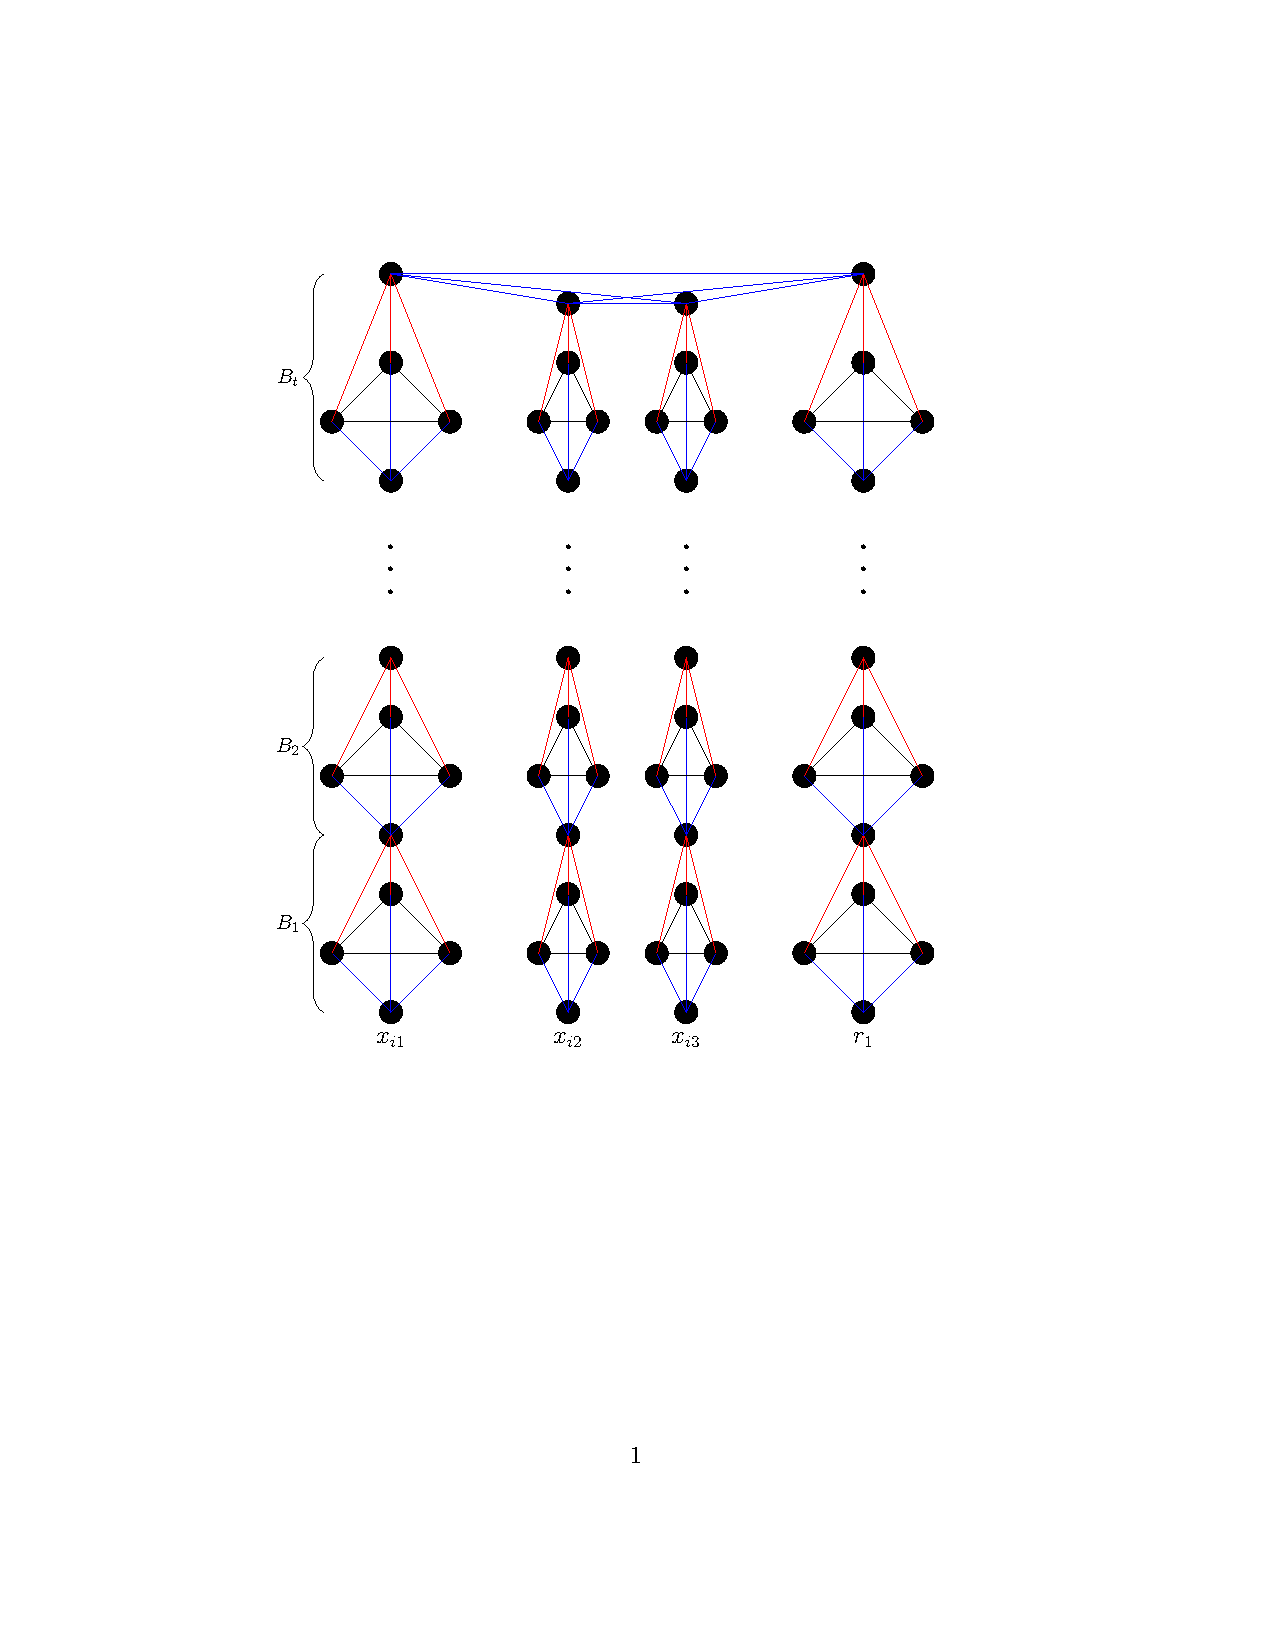
\includegraphics[trim = 100 290 100 100, clip, width=6cm, height=4.5cm]{figures/deDuplication/pccHard.pdf}
			\end{figure}
		\end{column}

		\begin{column}{0.48\textwidth}
		    Part of graph $G$ constructed by local replacement for the subset $S_i =  \{x_{i1}, x_{i2}, x_{i3}\}$. Illustration for $M = 4$.
		\end{column}
	\end{columns}

	
	\vspace{20pt}\begin{itemize}
		\item If $A$ outputs a clustering such that all clusters have size $M$ and no negative erros, then output YES.
		\vspace{10pt}\item Else NO.
	\end{itemize}
\end{frame}

\begin{frame}{Goals}
	Analyse the computation complexity of PCC.
	\begin{itemize}
		\vspace{10pt}\item NP-Hard.
	\end{itemize}	 
	\vspace{30pt}\alert{Can same-cluster queries make the problem easy}?	
\end{frame}

\begin{frame}{Hardness of PCC in the presence of an oracle}
	\begin{block}{Theorem}
		Given that the Exponential Time Hypothesis (ETH) holds. Any algorithm for PCC that runs in polynomial time makes $\Omega(|X|)$ same-cluster queries for all $M \ge 3$ and for $\alpha = 0$ and $\beta = \frac{1}{2}$. 
	\end{block}
	\onslide<2->
	\vspace{20pt}Strategy: Any algorithm for PCC takes $2^{\Omega(n)}$ time.
	\begin{itemize}
		\vspace{10pt}\item Any algorithm for X3C or equivalently 3DM takes $2^{\Omega(m)}$ time.
	\end{itemize}
\end{frame}

\begin{frame}{3SAT to 3DM}
	Classical constructions are `inefficient'.\\
	\begin{itemize}
	\vspace{10pt}\item \alert{[Johnson and Garey'79]} implies a query lower bound of $\Omega(|X|^{0.25})$.
	\end{itemize}
	
	\vspace{30pt}Linear reduction of independent interest.	
\end{frame}

\begin{frame}{Hardness: Linear reduction of 3SAT to 3DM}
	\begin{columns}
		\begin{column}{0.48\textwidth}
			\vspace{-40pt}\begin{figure}
				\centering
				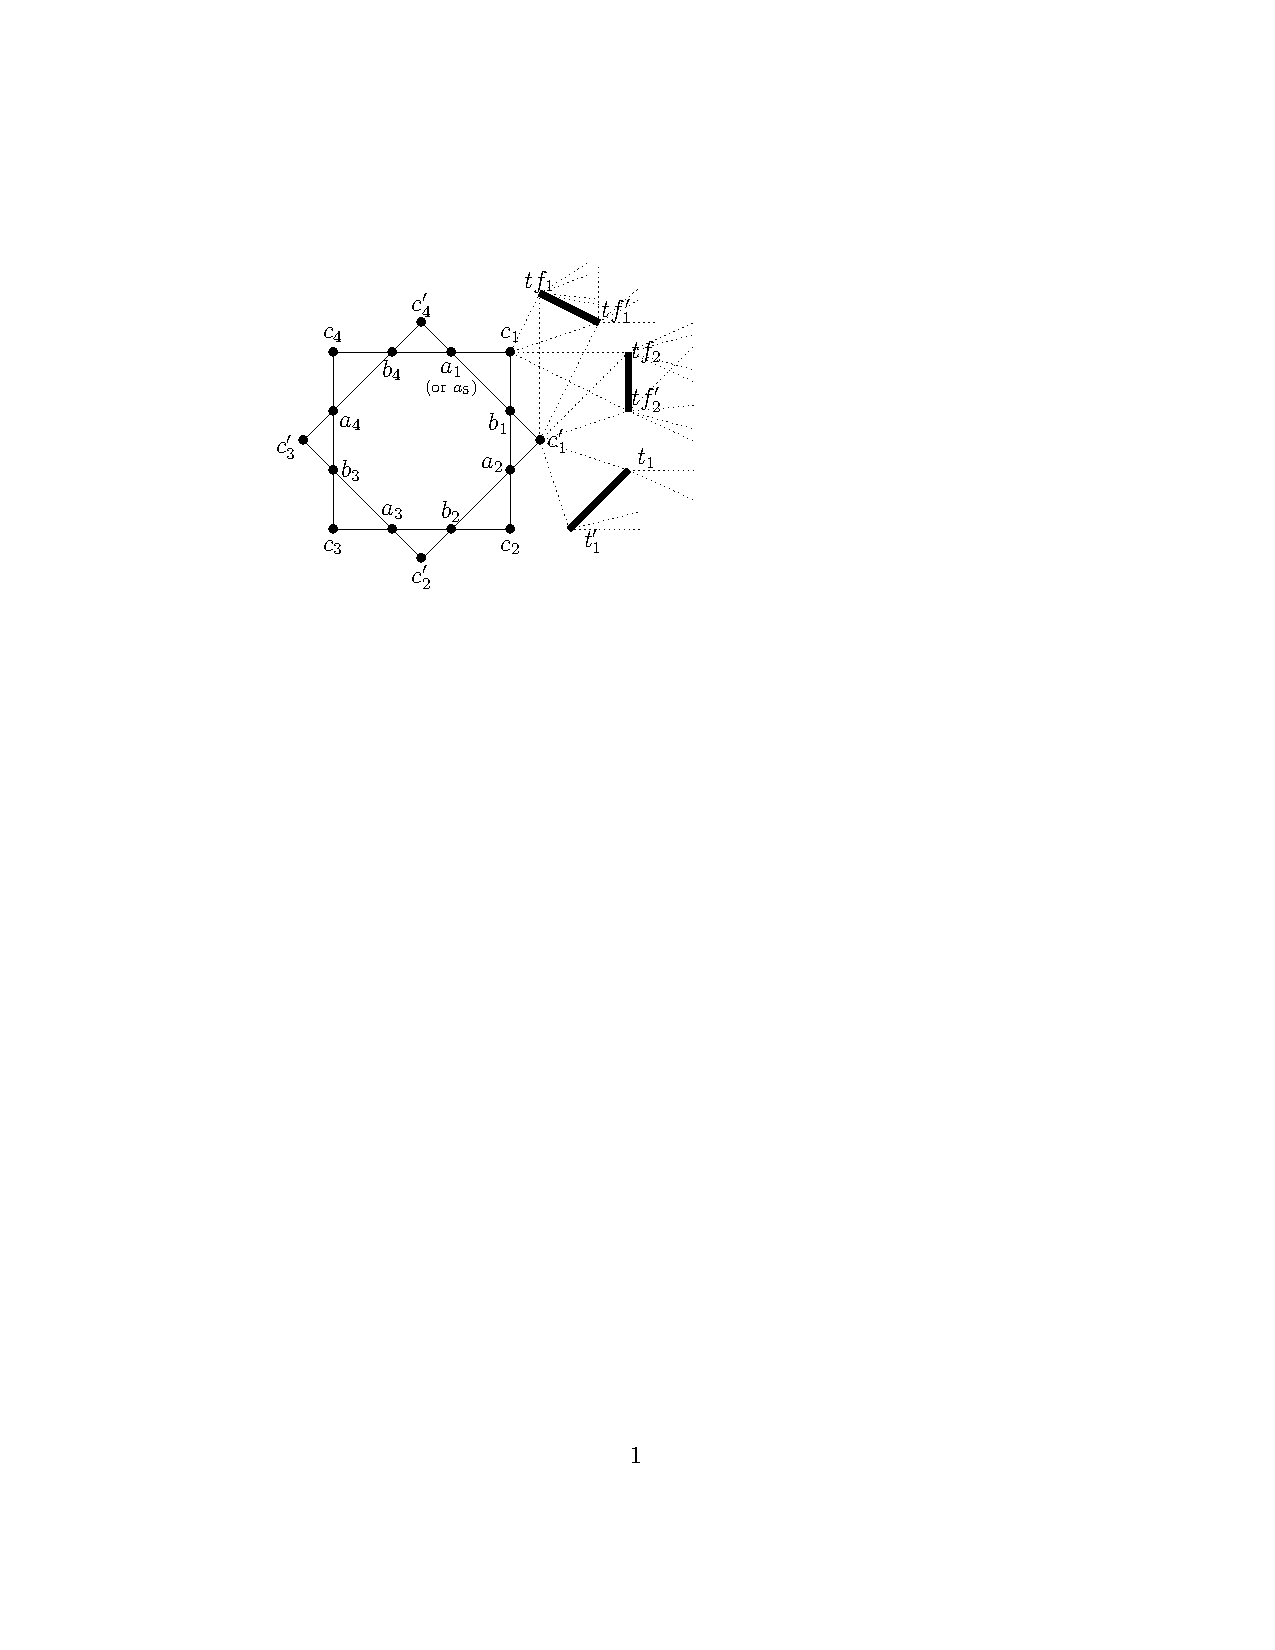
\includegraphics[trim = 120 500 300 120, clip, width=\linewidth]{figures/deDuplication/pccHardQuery.pdf}
			\end{figure}
		\end{column}

		\begin{column}{0.48\textwidth}
			\begin{itemize}
				\item Literal $x_1$ is part of four different clauses.
				\item $(a_i, b_i, c_i)$ capture truth assignment and $(b_i, c_i', a_{i+1})$ captures false assignment.
				\item Hyper-edges containing $tf_i, tf_i'$ and $t_1, t_1'$ capture truth setting for the clause $C = \{x_1, x_2, x_3\}$.
				
			\end{itemize}
		\end{column}
	\end{columns}	
	\begin{itemize}
		\item $t_1, t_1'$ ensure that atleast one of the literals is true. 
	\end{itemize}
\end{frame}

\begin{frame}{Goals}
	\Huge{
    \begin{center}
    	PCC is hard !!\\
    	\Frowny{} 
   	\end{center}
    }
\end{frame}

\begin{frame}{Circumventing the hardness?}
	Possible approach
	\begin{itemize}
		\item Design efficient approximation algorithms.		
	\end{itemize}
	
	\onslide<2->
	\vspace{30pt}Our approach
	\begin{itemize}
		\vspace{5pt}\item Limit the search space of clusterings $\mc F$.
		\vspace{5pt}\item Choose the best from a class of clusterings (or algorithms).
		\vspace{5pt}\item Useful tool for practitioners. 
	\end{itemize}
\end{frame}


\begin{frame}[label=RCC]{Restricted Correlation Clustering (RCC)}
	\begin{block}{Input}
		$(X, d)$, \hyperlink{RCCVariations}{class of clusterings} $\mc F$ and a $C^*$-oracle
	\end{block}
	
	\vspace{10pt}\begin{block}{Find}
		\vspace{-15pt}\begin{align*}
		  &\hat C = \argmin_{C \in \mc F} \enspace \text{correlation-loss}_{C^*}(C)
		\end{align*}	
	\end{block}
	
	\begin{block}{where}
		\vspace{-20pt}\begin{align*}
			d \text{ is }(\alpha, \beta)\text{-informative}&\\
			\text{correlation-loss}_{C^*}(C) &= \enspace  \mu \enspace \underset{(x, y) \sim P^+}{\mb P} \big[ C(x, y) = 0 ] \\
			&+\enspace (1-\mu) \enspace \underset{(x, y) \sim P^-}{\mb P} \big[ C(x, y) = 1] 
		\end{align*}
	\end{block}	
	$P^+$ is the uniform distribution over pairs where $C^*(x, y) = 1$
\end{frame}

\begin{frame}{Goal}
Analyse
	\begin{itemize}
		\vspace{15pt}\item Computational complexity
		\vspace{15pt}\item Query complexity
		\vspace{20pt}\item $\mc F = \{T_1, \ldots, T_s\}$ as a running example.\\
		\vspace{10pt}$T_i$ is a clustering tree.
	\end{itemize}
\end{frame}

\begin{frame}[label=RCCPositive]{Positive result}
	\begin{block}{}
		There exists sampling procedures \hyperlink{detailsRCCNegative}{$\mc P_0$} and \hyperlink{detailsRCCPositive}{$\mc P_1$} such that if an ERM algorithm receives $m_-$ and $m_+$ samples respectively where
		\vspace{-10pt}\begin{align*}
		  &m_-, m_+ \enspace \ge a\frac{\vcdim({\mc F}) + \log(\frac{3}{\delta})}{\epsilon^2} 
		\end{align*}
		then with probability atleast $1-\delta$, we have that $$L_{C^*}(\hat C) \enspace\le\enspace \min_{\mc C \in \mc F} L_{C^*}(C) + 3\alpha + \epsilon$$
	\end{block}

	\vspace{10pt}Computational and query complexity depends on
	\begin{itemize}
		\vspace{5pt}\item Time (and the number of queries) to  \alert{sample one point}. 
		\vspace{5pt}\item $m_-$ and $m_+$ (or the \alert{$\vcdim(\mc F)$}). 
	\end{itemize}		
\end{frame}



\begin{frame}[label=RCCVCDim]{VC-Dimension of common classes}
	\begin{block}{}
		Let \hyperlink{detailsRCCVCDim}{$\mc F = \{T_1, \ldots, T_s\}$} be a class of hierarchical clustering trees. Then 
		$$\vcdim({\mc F}) \in o(\log^2 s) $$
	\end{block}
	
	\begin{itemize}
		\vspace{20pt}\item $\vcdim(T)$ is upper bounded by a constant.
		\vspace{10pt}\item Using standard theorems that would imply $\vcdim(\mc F) \le O(s)$
	\end{itemize}
\end{frame}

\begin{frame}[label=CCTakeaways]{Key takeaways}
	\hyperlink{notesCCTakeaways}{For common classes of} clusterings, 
	\begin{itemize}
		\vspace{20pt}\item ERM-based approach can solve the RCC problem efficiently. 
		\vspace{15pt}\item Time and query complexity of RCC depend on the richness of $\mc F$.
	\end{itemize}
\end{frame}

\begin{frame}[label=RCCExperiments]{Experiments}
	\begin{figure}
	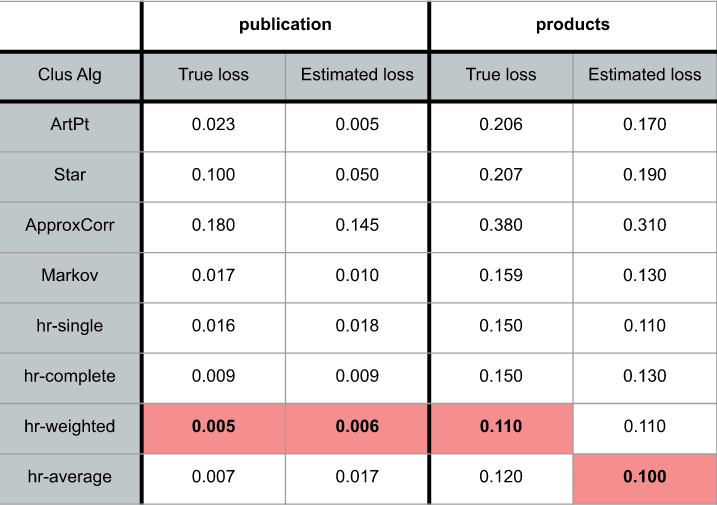
\includegraphics[trim=0 0 0 0,scale=0.35]{figures/deDuplication/experimentsMain.png}
	\caption{\hyperlink{detailsRCCExperiments}{Evaluation of different algorithms on different datasets} using our framework.}
	\end{figure}
\end{frame}

\begin{frame}<2>{Outline}	
	\onslide<1>End of first part
	\vspace{10pt}\begin{block}{}
	\mynum{2} Under-specificity \alert{and} \\\vspace{10pt}\mynum{1} Computational complexity
	\end{block}
		
	\onslide<2>\vspace{35pt}Second part
	\vspace{10pt}\begin{block}{}
	\mynum{3} Noise-robustness \alert{and} \\\vspace{10pt}\mynum{1} Computational complexity
	\end{block}		
\end{frame}


\begin{frame}[label=noiseFramework]{High-level problem definition}

	Input: $(X, d)$
	\vspace{20pt}
	
	Assuming the data consists of 
	\begin{itemize}
	\vspace{5pt} \item \hyperlink{notesClusterability}{Structured subset $S$ - Has a ``nice''} clustering.  
	\vspace{5pt} \item Unstructured complement $N = X \setminus S$
	\end{itemize}

	\vspace{20pt}
	{\color{blue} Output} a partition $C=(C_1, \ldots C_k)$ of $X$.
	\begin{itemize}
		\vspace{5pt}\item $C|_{S} $ \emph{induces} a ``nice'' clustering of $S$. 
	\end{itemize}

	\vspace{20pt} Algorithm is robust to noise of type $N$.
\end{frame}

\begin{frame}{Clustering in the presence of sparse noise}
	\begin{itemize}
		\item Joint work with Samira Samadi and Shai Ben-David.
		\vspace{20pt}\item In proceedings of \alert{ALT'16}. 
	\end{itemize}
\end{frame}

\begin{frame}{Sparse noise}
	\begin{itemize}
		\item Noise doesn't pretend to be a cluster.
		\vspace{20pt}\item Any ``small'' ball doesn't contain ``many'' noisy points.
	\end{itemize}
\end{frame}

\begin{frame}{Definitions}

	Given $(X, d)$, a set $S \subseteq X$\\
	\vspace{10pt}A clustering $\mc C = \{S_1, \ldots, S_k\}$ of the set $\mc S$ induced by centers $s_1, \ldots, s_k \in X$.

	\vspace{10pt}\begin{block}{$(\alpha, \eta)$-center proximity}
	\vspace{0.5cm} {\bf $\alpha$-center proximity}: For all $x \in S_i$ and $i\neq j$, $$\alpha d(x, s_i) < d(x, s_j)$$
	{\bf $\eta$-sparse noise}: For any ball $B$, 
	$$r(B)\leq \eta \thinspace r(\mc{C}) \implies |B\cap (\mc X\setminus \mc S)| < \frac{m(\mc C)}{2}$$
	\end{block}
\end{frame}


\begin{frame}[label=positiveSarseNoise]{Positive result}
	\begin{block}{}
		We \hyperlink{detailsPositiveSparseNoise}{construct in polynomial time a clustering} tree $T$ such that for all $k$, for all $S \subseteq X$ and for all $k$-clusterings $C_S$, if 
	  	\begin{itemize}
	  		\item $C_S$ satisfies \alert{$(2+\sqrt{7}, 1)$}-center proximity
	  		\item Runs in time $O(|X|^3)$.
	  	\end{itemize}
	  	then $T$ captures $C_S$.
  	\end{block}
  	
	\begin{figure}
	  \includegraphics[trim = 0 0 0 200, scale=0.4]{figures/clusteringNoise/hier.pdf}
	\end{figure}	  	
\end{frame}

\begin{frame}[label=negativeSparseNoise]{Negative results}
	\begin{block}{}
  \begin{itemize}
  	\vspace{10pt}\item \hyperlink{detailsNegativeSparseNoise}{For \alert{$\alpha < 2 +\sqrt{3}\approx 4.4$} and $\eta \le 1$ there does not exist a }tree which can capture all $(\alpha, \eta)$-proximal clusterings. 
	\vspace{20pt}\item For \alert{$\alpha < 2\sqrt{2} + 3 \approx 5.8$} and adversarial noise there does not exist a tree which can capture all $\alpha$-proximal clusterings if the number of noisy points exceed $\frac{3m(C_S)}{2}$. 
	\end{itemize}	 
	\end{block}
\end{frame}

\begin{frame}{Key Takeaways}
	\begin{itemize}
		\item Notion of sparse noise to handle background noise.
		\vspace{25pt}\item Efficient hierarchical algorithm that captures {\color{blue}all nice} solutions.
		\vspace{25pt}\item Positive result {\color{blue}independent} of the number of noisy points.
	\end{itemize}
\end{frame}

\begin{frame}{Noise-robust clustering objectives}
	\begin{itemize}
		\item Joint work with Yaoliang Yu and Shai Ben-David.
		\vspace{25pt}\item Available on \alert{arxiv'17}. 
	\end{itemize}
\end{frame}

\begin{frame}[label=optimizationNoise]{Summary}
	\begin{block}{\hyperlink{detailsOptimizationNoise}{$\lambda$-regularized paradigm}}
		$$\sum_{i =1}^k\enspace\sum_{x \in C_i} \|x - \mu_i\|^2 \enspace+\enspace \textcolor{red}{\lambda |C_{k+1}|}$$
	\end{block}
	
	\begin{center}$\Downarrow$\end{center}
	
	\begin{block}{}
		\begin{center}SDP Relaxation\end{center}
	\end{block}
	
	\begin{center}$\Downarrow$\end{center}
	
	\begin{block}{}
		SDP Relaxation is tight under the \alert{`noisy' stochastic ball} model.
	\end{block}
		
\end{frame}

\begin{frame}
    \Huge{\centerline{Thank You!}}
\end{frame}

%----------------------------------------
%        Figure Samples
%----------------------------------------


\begin{frame}[label=notesIntroduction]{Notes: Introduction}
\hyperlink{clusteringChallenges}{$k$-means}
\begin{itemize}
  \item NP-Hard for $k = 2$ and $d = n$. $[$Dasgupta' 08$]$
  \item NP-Hard for $k = n^{\epsilon}$ and $d = 2$. $[$Vattani' 09$]$
  \item NP-Hard to approximate within $(1+\epsilon)$
\end{itemize}
$k$-median \{centers in metric space (84) and remaining from data.\}
\begin{itemize}
	\item NP-Hard for $k=\Omega(n)$ and $d=2$ $[$Megiddot and Supowit '84$]$.
	\item $(3+\epsilon)$-approximation $[$Arya et. al'01$]$
	\item $(1+\sqrt3 + \epsilon)$-approximation $[$Li and Svensson '12$]$
\end{itemize}
$k$-center (maximum of $l1$ distances)
\begin{itemize}
	\item NP-Hard to approximate within constant $[$Megiddot and Supowit '84$]$ for $k=\Omega(n)$ and $d=2$
\end{itemize}
\end{frame}

\begin{frame}[label=notesUnderspecificityRelated]{Notes: Under-specificity related work}
\hyperlink{underspecificityRelated}{Incoporating domain knowledge}
\begin{itemize}
  \item $[$Wagstaff et. al '01$]$\\
  Must/cannot link constraints are provided as input.\\ 
  Constrained k-means - Each point is assigned to the closest center such that the constraints are satisfied. 
  \item $[$Ashitiani, Ben-David '15$]$\\
  Cluster a small subset and learn a consistent model.\\
  Mapping under which $k$-means is close to the target clustering.\\
  Sample complexity analysis.
  \item $[$Balcan, Blum '08$]$\\
  Merge-split queries.\\
  Given a class $C$ of clusters, recover the target clustering.\\
  A generic but inefficient procedure which makes $O(k^3 \log |C|)$ queries.
  \end{itemize}
\end{frame}

\begin{frame}[label=notesMergeSplitQueryRelated]{Notes: Merge-Split query related work}
\hyperlink{underspecificityRelated}{[Awasthi, Balcan, Voevodski '17]}
\begin{itemize}
  \item Clustering recovery by making  atmost $O(\delta)$ merge-split queries where $\delta$ is the error of initial clustering. 
  \item Over-clustering and under-clustering errors are upper bounded by $k^2$.
  \item For CC, if the initial clustering has error $\delta$ (number of incorrect edges $O(n)$) - Recovers by making atmost $\delta$ queries.
  \end{itemize}
\hyperlink{underspecificityRelated}{[Balcan et. al '18]}
\begin{itemize}
  \item Finite set $P$ of clustering instances and a distribution $D$ over them. Any algorithm $h$ on a clustering instance $X$ incurs a cost given by $cost(h, X)$. The goal is to find algorithm $h'$ such that
$$E [ cost(h',  X) ]    -   min_{h \in H}   E [cost(h, X)]   < \epsilon$$
\item If $P$ is just one instance then we should see all the labels. In this case, their `learning' algorithm is actually solving a computational problem of how to approximately (and efficiently) find the best algorithm.  
\end{itemize}
\end{frame}

\begin{frame}[label=resultsGammaMargin]{Results: Gamma Margin}
  \hyperlink{gammaMargin}{Given}: $X$ and $k$\\
  \vspace{10pt}Optimal solution to the desired objective function satisfies $\gamma$-margin.

	\begin{table}[]
	\centering
	%\caption{My caption}
	\label{my-label}
	\begin{tabular}{lll|lll|}
	& $k$-means &  &  &    & \begin{tabular}[c]{@{}l@{}}Poly-time solvable for $\gamma \ge 3$\\ NP-Hard for $\gamma < 3$\end{tabular} \\\\
	\hline\\
	& $k$-median &  &  &  & \begin{tabular}[c]{@{}l@{}}Poly-time solvable for $\gamma \ge 2$\\ NP-Hard for $\gamma < 2$\end{tabular}
	\end{tabular}
	\end{table}
	
	\begin{itemize}
		\item $\gamma \ge 3$ - Single-linkage
		\item $\gamma < 3$ - Max-$k$-coverage problem
		\item $\gamma \ge 2$ - Hierarchical approach where distance between two clusters is radius of smallest ball containing them.
		\item $\gamma < 2$ - Perfect dominating set promise problem.
	\end{itemize}
\end{frame}

\begin{frame}[label=resultQueryPositive]{Positive result: Same-cluster query}

	\begin{block}{\hyperlink{queryPositive}{The algorithm}}
	1. Estimate center
	\begin{itemize}
		\item Query uniformly till we have ``enough'' points from one cluster
    \end{itemize}  
	2. Compute radius
	\begin{itemize}
	  \item Binary search to find the ``radius"
    \end{itemize}  	
	3. Delete and repeat
  \end{block}
  Proof
  \begin{itemize}
	\item If $d(\mu, \mu') \le \epsilon$ and $\gamma > 1 + 2\epsilon$, then $d(x, \mu') < d(y, \mu')$. Hence, there is a separation even w.r.t to the center $\mu'$.

	\item Concentration inequality in high dimensions. Namely, if $n > c\frac{\log (1/\delta)}{\epsilon^2}$ then $\|\mu - \frac{1}{n}\sum X_i\|^2 \le R^2 \epsilon$ 
  \end{itemize}
\end{frame}

\begin{frame}[label=resultQueryNegative]{Hardness result: Same-cluster query}
\hyperlink{queryNegative}{Proof ideas}
\begin{itemize}
\item Any clustering of $X$ which costs $\le L$ has the following property. \item Atleast $m$ of rows $R_i$ are be grouped in a $A$-type clustering and the rest are grouped in $B$-type clustering. 
\item The rows of $G_i$ are singletons. 
\item And the points in $Z_i$ are added to clusters which are good for it (increase the cost by $\frac{2}{\sqrt{3}}h$. 
\item Other clusterings have cost atleast $L + \frac{w}{3}$. 
\item If $S_i = (s_{i1}, s_{i2}, s_{i3})$ is included in the exact cover then the row $R_i$ should be grouped in a $A$-type clustering. 
\item Then $x'_{ij}$ location will force all other dash locations to be in $B$-type clusterings (as the up ones will have to go `up' and the down ones will have to go down). 
\item Since there are $3m$ variables they will have exactly $m$ rows in $A$-type clustering.
\end{itemize}
\end{frame}

\begin{frame}[label=notesQueryTakeaways]{Notes: Same-cluster queries}
	\hyperlink{queryTakeaways}{Other avenues}
	\begin{itemize}
		\item Approximate $k$-means clustering
		\item $k$-median and $k$-center clustering under same-cluster queries.
		\item Clustering with noisy oracles.
		\item Queries in mixture models.
		\item Correlation clustering.
	\end{itemize}
\end{frame}

\begin{frame}{Notes: Same-cluster queries}
	\hyperlink{queryTakeaways}{Semi-supervised learning}
	\begin{itemize}
		\item Generative models
		\item Supervised-SVM
		\item Mincut
		\item Harmonic functions
	\end{itemize}
\end{frame}

\begin{frame}[label=notesCC]{Notes: Correlation Clustering}
	\hyperlink{CC}{Designing a distance} metric
	\begin{itemize}
		\item Character-based: Edit distance and its many variants.
		\item Token-based: Word representations. Word2vec or tf-idf measures.
		\item Phonetic-based: Soundex, NYSIIS. Replace similar sounding constants with numbers or letters.
		\item Numerical
	\end{itemize}
	Learning a distance metric.
	\begin{itemize}
		\item Learning the weights of (distance functions across) different fields.
		\item Learning a classifier over pairs. (Can view as a $\{0, 1\}$ distance function.)
	\end{itemize}
\end{frame}

\begin{frame}[label=notesCCHardness]{Notes: Hardness of Correlation Clustering}
	\begin{itemize}
	\item $[$Bansal et al., 2004$]$\\
	\hyperlink{CC}{Constant} factor approximation. Constant is huge. 
	\item $[$Demaine et al., 2006$]$\\
	$4\log_2 n$-approximation. $O(\log_2 n)$ approximation to weighted CC.\\
	APX-Hard for general weighted or unweighted graphs.
	\item $[$Charikar et al., 2005$]$\\
	Factor $4$ approximation to the minimization problem.\\
	Also, proved that the problem is APX-Hard. 
	\item $[$Giotis and Guruswami, 2006$]$\\
	PTAS when $k$ is known. Running time is $n^{O(\frac{9^k}{\epsilon^2})}\log n$.	
	\item $[$Ailon et al., 2018$]$\\
	Algorithm makes $O(\frac{k^{14} \log k\log n}{\epsilon^6})$ queries  and finds a $(1+\epsilon)$-approx. \\
	$(1+\epsilon)$-approximation makes $\Omega(\frac{k}{poly(\log k)})$ queries. 
\end{itemize}
\end{frame}

\begin{frame}[label=RCCVariations]{RCC Variations}
	\hyperlink{RCC}{Input}: $X$\\
	Distance: $d$ over $X^2$.\\
	A class of clusterings: $\mc F$\\
	
	Construct $G = (X, E)$, 
	
	\vspace{10pt}Output: 
	\vspace{-10pt}\begin{align*}
	  &\hat C = \argmin_{C \in \mc F} \enspace \text{correlation-loss}_{E}(C)
	\end{align*}
	Iterate over clusterings in $\mc F$		
	\begin{itemize}
		\item Bottom-up traversal when $\mc F = \{T_1, \ldots, T_s\}$.
	\end{itemize}
	Choose the one with smallest loss.
\end{frame}

\begin{frame}[label=CCThoughts]{Thoughts on different variations of CC}
	\hyperlink{CCFramework}{Solving $L_E(C)$ does not help} us solve $L_{C^*}(C)$\\
	$\alpha = 0$ and $\beta = \frac{1}{2}$. In this case, all the negative edges are correct and half of the positive edges are correct.\\
	Graph can be decomposed into cycles of length four.\\
	For every solution to $L_E(C)$ there exists a $C^*$ such that $L_{C^*}(C)$ is `bad'. 
\begin{table}[!ht]
\centering
\def\arraystretch{1.5}
\begin{tabular}{c|c}
	All possible clusterings & Restricted to $F$\\
	\hline
	Find $C^* = \text{argmin } L_{C^*}(C)$ & $\hat C = \text{argmin } L_{C^*}(C)$ \\
	vaccous equivalent to ``Find $C^*$ & \\
	\hline 
	Find $C^* = \text{argmin } L_{E}(C)$ & $\hat C = \text{argmin } L_{E}(C)$\\
	optimal solution is the desired clustering.\\
	\hline
\end{tabular}
\end{table}
\end{frame}

\begin{frame}[label=notesInformativeMetric]{Notes: Informative metric}
	\begin{table}[!ht]
\centering
\def\arraystretch{1.5}
\begin{tabular}{c|c|c|c}
	& \multirow{2}{2cm}{\hyperlink{informativeMetric}{Condition positive}} & \multirow{ 2}{1cm}{Condition negative}&\\
	&&&\\
	Predicted positive &tp &fp & \multirow{2}{3cm}{$precision = \frac{tp}{tp+fp}$}\\
	predicted negative &fn & tn\\
	\hline
	& $recall = \frac{tp}{tp+fn}$& $specificity = \frac{fp}{fp+tn}$ &
\end{tabular}
\caption{Precision and recall table}
\end{table}
\noindent $(\alpha, \beta)$-informative says that the edges $E$ and $C^*$ have high precision and recall w.r.t each other.  
\end{frame}

\begin{frame}[label=notesCCTakeaways]{Notes: CC Takeaways}
	\begin{itemize}
	\item $[$Claire Mathieu and Warren Schudy, 2010$]$ \\
	Correlation clustering under a semi-random model. \\
	A planted clustering and edges flipped independently with probability $p$. \\
	On complete graphs finds a clustering of cost $1+O(n^{-\frac{1}{6}})$ times the optimal. 
	\item $[$Mazumdar and Saha '17$]$\\
	Recover all clusters of size $\min\{k, \sqrt n\}\log n$\\
	Relation to noisy oracles.
	\end{itemize}
\end{frame}

\begin{frame}[label=detailsRCCNegative]{$\mc P_0$: Sampling negative pairs}
	
	\vspace{10pt}\textcolor{blue}{\hyperlink{RCCPositive}{Basic Idea}}\\
	Sample (with rejection) uniformly at random from $X^2$. 
	
	\vspace{20pt}\begin{block}{Results}
		\begin{itemize}
			\vspace{5pt}\item Samples a pair according to $P^-$ in $O(1)$ expected time.
			\vspace{10pt}\item Makes $\frac{1}{1-\gamma}$ queries to the oracle in expectation. 
		\end{itemize}			
	\end{block}
	
	
\end{frame}

\begin{frame}[label=detailsRCCPositive]{$\mc P_1$: Sampling positive pairs}
	
	\vspace{20pt}\textcolor{blue}{\hyperlink{RCCPositive}{Basic Idea}}\\
	Sample (with rejection) uniformly at random from the set of `close' points. $K = \{(x, y): d(x, y) \le \lambda\}$. 

	\vspace{10pt}\begin{block}{Results}
		\begin{itemize}
			\vspace{5pt}\item Samples a pair according to $T$ which $2\alpha$-approximates $P^+$.
			$$\Big|\underset{(x, y) \sim P^+}{\mb P}\enspace \big[ h(x, y) = 0 ] - \underset{(x, y) \sim T}{\mb P}\enspace \big[ h(x, y) = 0 ]\Big|  \enspace \le \enspace 2\alpha.$$ 
			\vspace{5pt}\item Makes $\frac{1}{\beta}$ queries to the oracle in expectation. 
		\end{itemize}			
	\end{block}
\end{frame}

\begin{frame}[label=detailsRCCPositiveLSH]{$\mc P_1$: Faster sampling LSH-able metrics}
		\vspace{20pt}\alert{$\Theta(n^2)$} time to construct set $K$.	

	\vspace{20pt}Use an \hyperlink{RCCPositive}{LSH scheme to `approximately construct' $K$}.
 	\begin{itemize}
		\vspace{5pt}\item Obtain $s$ different partitions of $X$.
		$$ B := \{P_1, \ldots, P_s\} = \{B_{ij} : 1\le i\le s, 1\le j \le |P_i|\}$$
	\end{itemize}	
\end{frame}


\begin{frame}{$\mc P_1$ results for LSH-able metrics}
	\textcolor{blue}{Basic Idea}\\
	\hyperlink{RCCPositive}{Sample (with three-step rejection) uniformly} at random from $B$.
	\begin{itemize}
		\vspace{5pt}\item Reject with probability $= 1 - \frac{1}{\text{ \#blocks in which the pair occur together}}$
		\vspace{5pt}\item Reject based on distance and then the oracle.
	\end{itemize} 
	
	\begin{block}{Results}
		\begin{itemize}
			\item $T$ which approximates $P^+$ (with high probability).
			\begin{align*}
  &\Big|\underset{(x, y) \sim P^+}{\mb P} \big[ C(x, y) = 0 ] -\underset{(x, y) \sim T}{\mb P} \big[ C(x, y) = 0 ] \Big| \le 2\alpha + \zeta  + \nu
  			\end{align*} 
			$\zeta$ depends on hashing and $\nu$ controls the success probability. 
			\vspace{10pt}\item Makes $O(\frac{1}{\beta})$ queries to the oracle in expectation. 
		\end{itemize}			
	\end{block}
\end{frame}

\begin{frame}[label=detailsPositiveSparseNoise]{Clustering under $(\alpha, \eta)$-center proximity}
	\begin{block}{The algorithm}
	  \vspace{10pt}\hyperlink{positiveSparseNoise}{Input: $(X, d)$ and a parameter} $t$.\\

	  \vspace{20pt}For all pairs $p, q$ in increasing order of distance.\\
	  \vspace{10pt}If $B := B(p, d(p, q))$ satisfies the \alert{sparse-distance condition}
	  \begin{itemize}
	  	\vspace{5pt}\item Merge all clusters that intersect with $B$ into a single cluster
	  \end{itemize}
    \end{block}

\end{frame}


\begin{frame}{Sparse-distance condition}
    \hyperlink{positiveSparseNoise}{All clusters that intersect with $B$ should have a non-sparse intersection}. 
	\begin{itemize}
	  \item $|B| \ge t$.
	  \item For any $X_i \in \mc C$, if $X_i \cap B \neq \emptyset$, then $X_i \subseteq B$ or $|B \cap X_i| \ge t/2$.
	\end{itemize}

   \begin{figure}
   	  \centering
	  \includegraphics[scale=0.3]{figures/clusteringNoise/3.pdf}
	  \includegraphics[scale=0.3]{figures/clusteringNoise/4.pdf}
   \end{figure}
\end{frame}

\begin{frame}[label=detailsNegativeSparseNoise]{Details: Lower bound under sparse noise}
	\hyperlink{negativeSparseNoise}{If $\alpha < 3 + \sqrt{2}$ and noise is sparse}
	\begin{itemize}
		\item No clustering tree can capture all nice solutions.
	\end{itemize}
	
	\vspace{20pt}\begin{figure}[!t]
	  \begin{center}
	    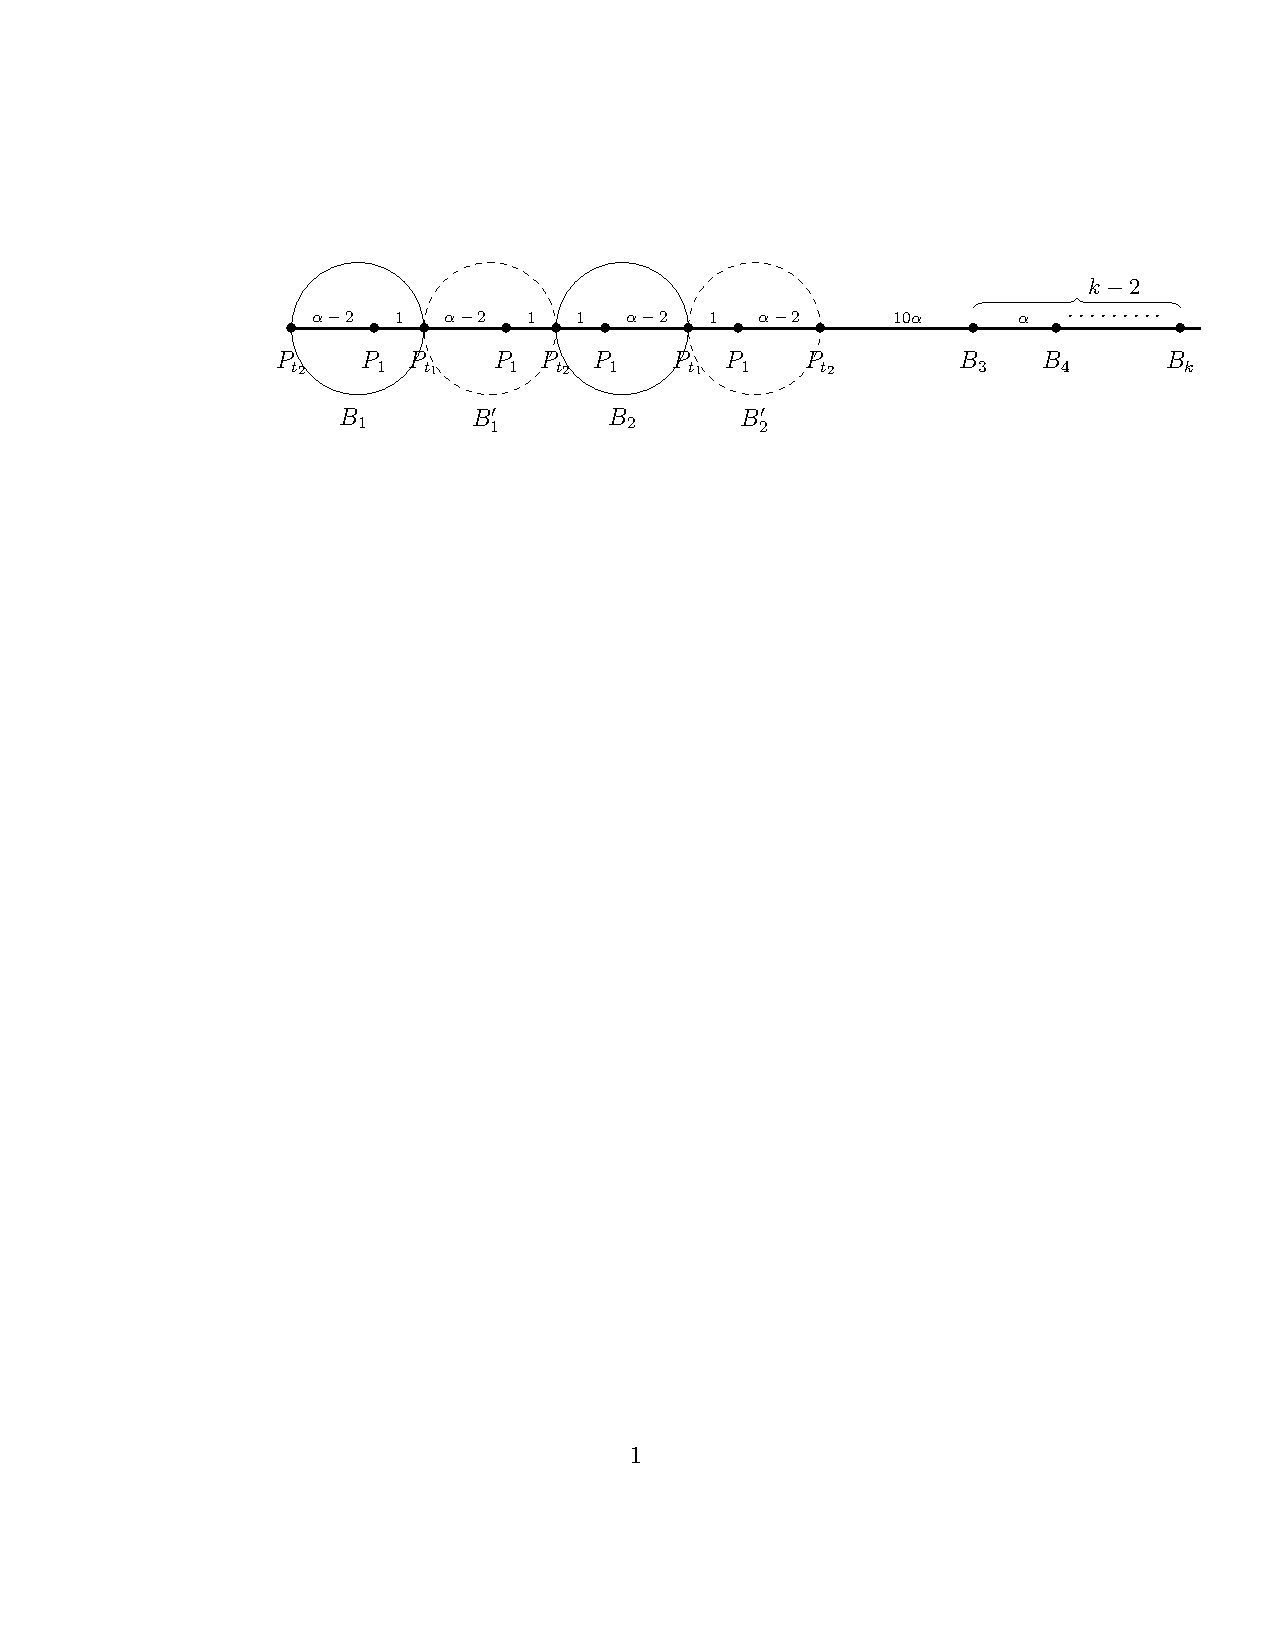
\includegraphics[trim={47mm 205mm 12mm 44mm},clip,width=\textwidth]{figures/clusteringNoise/lbdFig2.pdf}
	  \end{center}
	\end{figure}
	\vspace{20pt}Same ideas can be extended to a list output.\\
	\begin{itemize}
		\item Any list should have size $> 2^{k/2}$
	\end{itemize}
\end{frame}

\begin{frame}[label=detailsOptimizationNoise]{Robustifing clustering objectives}
	\hyperlink{optimizationNoise}{$\lambda$-regularized paradigm}.
	\begin{itemize}
		\vspace{5pt}\item $$\sum_{i =1}^k\enspace\sum_{x \in C_i} \|x - \mu_i\|^2 \enspace+\enspace \textcolor{red}{\lambda |C_{k+1}|}$$
		\vspace{20pt}\item Discard points into a garbage cluster.
	\end{itemize}
	
	\vspace{20pt}\textcolor{blue}{Can regularization help with noise-robustness?}
\end{frame}

\begin{frame}{Sidenote: Properties of the regularized $k$-means objective}	
	\hyperlink{optimizationNoise}{For all $\lambda$}
	\begin{itemize}
		\item For all clustering instances 
		\begin{itemize}
			\vspace{10pt}\item Easy for $\lambda \le \frac{m(X)}{2}$.
			\vspace{10pt}\item Reduces to classical $k$-means for $\lambda \ge \frac{M(X)}{2}$.			
		\end{itemize}
		\vspace{20pt}\item There exists instance which are NP-Hard for $\textcolor{blue}{k \ge 1}$ if $$\frac{m(X)}{2} < \lambda$$
	\end{itemize}
\end{frame}

\begin{frame}{Tackling computational hardness}
	$$\text{Original objective} \longrightarrow \text{Convex relaxation}$$
	
	\vspace{20pt}Tightness under the {\color{blue}stochastic ball assumption}.
	\begin{itemize}
		\vspace{10pt}\item $k$ unit balls separated by $\delta$
		\vspace{10pt}\item Generated by isotropic distribution. 
	\end{itemize}	
\end{frame}

\begin{frame}{Previous work under the stochastic ball model}
	\begin{table}
		\centering
		\label{table:stochasticBall}
		\setlength{\tabcolsep}{0.7em} 
		{\renewcommand{\arraystretch}{1.5}%
		\begin{tabular}{llc}
		\\
		 & Separation condition & Reference\\
		 \hline
		$k$-median LP & $\delta > 3.75$ & \alert{[Nellore et. al' 15]}\\
		 & $\delta > 2$ & \alert{[Awasthi et. al'15]}\\
		\hline
		$k$-means LP & $\delta > 4$ & \alert{[Awasthi et. al'15]}\\
		\hline
		$k$-means SDP & $\delta > 2\sqrt2 (1 + \frac{1}{\sqrt d})$ & \alert{[Awasthi et. al'15]}\\
		 & $\delta > 2 + \frac{k^2}{d}cond(\gamma)$ & \alert{[Iguchi et. al'15]}\\
		 & $\delta > 2 + \frac{k^2}{d}$ & \alert{[Iguchi et. al'17]}\\

		\label{table:alphacenter}
		\end{tabular}
		}
	\end{table}
\end{frame}

\begin{frame}{SDP-based relaxation}
	Equivalence of the regularized objective 
	$$\sum_{i =1}^k\enspace\sum_{x \in C_i} \|x - \mu_i\|^2 \enspace+\enspace \lambda |C_{k+1}|$$ to the following.
	
	$$	
	\text{0-1 SDP}
	\begin{cases}
		\min_{Z, y} \enspace &\tr(DZ) + \lambda \langle \mb 1, y\rangle\\
		\text{s.t. } \enspace &\tr(Z) = k\\
		& Z\cdot \mb 1 + y = \mb 1\\	
		&Z\ge 0, Z^2 = Z, Z^T = Z \\
		& y \in \{0, 1\}^n
	\end{cases}	
	$$
\end{frame}

\begin{frame}{SDP-based relaxation}
	\hyperlink{optimizationNoise}{Relaxation of the regularized} objective gives
	$$	
	\text{Regularized SDP}
	\begin{cases}
		\min_{Z, y} \enspace &\tr(DZ) + \lambda \langle \mb 1, y\rangle\\
        \text{s.t. } \enspace &\tr(Z) = k\\
		& \Big(\frac{Z+Z^T}{2}\Big)\cdot \mb 1 + y = \mb 1\\		
		&Z \ge 0, y \ge 0\\
		& Z \succeq 0
	\end{cases}
	$$
\end{frame}

\begin{frame}{Main result}
	\begin{theorem}
	 If  
	\begin{itemize}
	  \item $\delta > 2 + \sqrt{ O(\zeta) + \frac{k}{d}}$ 
	  %\item $\alpha \ge O(\zeta)+ \frac{k}{d}$ 
	  %\item $\frac{|N_2|}{n} \le \frac{\delta^2-2\delta-O(\zeta)}{\lambda}$	  
	\end{itemize}
	\hyperlink{optimizationNoise}{and the noise satisfies certain mildness conditions (relative to the size and} distance to $S$) then the regularized $k$-means SDP outputs the clustering $C$ such that
	$$C|_{S} = \{B_1, \ldots, B_k\}$$
	%Let $n = \min_i |B_i|$ and $\zeta = \frac{|N_1|}{n}$. 
	\end{theorem}
	
	\vspace{20pt}{\color{blue}Corollary}\\
	For the noiseless case, the $k$-means SDP finds the desired clustering for $$\delta > 2 + \sqrt{\frac{k}{d}}$$
\end{frame}

\begin{frame}[label=detailsRCCExperiments]{Details: Experiments for RCC}
	\begin{figure}
	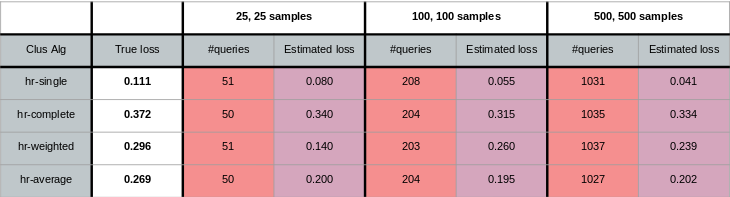
\includegraphics[trim=0 0 0 0,scale=0.4]{figures/deDuplication/experimentsQueries.png}
	\caption{\hyperlink{RCCExperiments}{Effect of number of queries on estimates} using queries.}
	\end{figure}
\end{frame}

\begin{frame}{Details: Experiments for RCC}
	\begin{figure}
	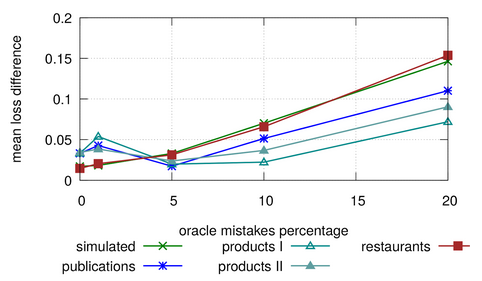
\includegraphics[trim=0 0 0 0,scale=0.5]{figures/deDuplication/experimentsNoisyOracle.png}
	\caption{\hyperlink{RCCExperiments}{Effect of oracle errors } on the results obtained using our framework.}
	\end{figure}
\end{frame}

\begin{frame}[label=notesClusterability]{Notes: Clusterability assumptions}
	\begin{itemize}
		\item $(\alpha, \epsilon)$-center proximity\\
		 \hyperlink{noiseFramework}{Efficient} $(1+\frac{8n}{m(C)}\epsilon)$-approximation to the $k$-median objective for $\alpha > 2 + \sqrt{7}$.
		 
		 \item $\epsilon$-separatedness\\
		 $Cost(OPT(k)) \le \epsilon^2 Cost(OPT(k-1))$. Variant of $k$-means finds a $(1+\epsilon)$-approximation with high probability in time $O(nk+k^3)$. \\
		 For $k=2$, algorithm succeeds with probability $1-\frac{20\epsilon^2}{\sqrt{(1-\epsilon^2)(1-101\epsilon^2)}}$. This implies average radius much smaller than separation.
		 $r_i < \frac{\epsilon}{\sqrt{1-\epsilon^2}} d(c_i, c_j)$.  
	\end{itemize}
\end{frame}

\end{document}



